% Options for packages loaded elsewhere
\PassOptionsToPackage{unicode}{hyperref}
\PassOptionsToPackage{hyphens}{url}
%
\documentclass[
  10pt,
]{article}
\usepackage{lmodern}
\usepackage{setspace}
\usepackage{amssymb,amsmath}
\usepackage{ifxetex,ifluatex}
\ifnum 0\ifxetex 1\fi\ifluatex 1\fi=0 % if pdftex
  \usepackage[T1]{fontenc}
  \usepackage[utf8]{inputenc}
  \usepackage{textcomp} % provide euro and other symbols
\else % if luatex or xetex
  \usepackage{unicode-math}
  \defaultfontfeatures{Scale=MatchLowercase}
  \defaultfontfeatures[\rmfamily]{Ligatures=TeX,Scale=1}

% Set roman back to Spectral for serifs
\setromanfont[Path = .pandoc/fonts/,
             Extension = .ttf,
             UprightFont       = *-Regular ,
             BoldFont          = *-Bold ,
             ItalicFont        = *-Italic ,
             BoldItalicFont    = *-BoldItalic ,
             Ligatures=TeX]{IBMPlexSerif}
\setsansfont[Path = .pandoc/fonts/,
             Extension = .ttf,
             UprightFont       = *-Regular ,
             BoldFont          = *-Bold ,
             ItalicFont        = *-Italic ,
             BoldItalicFont    = *-BoldItalic ,
             Scale             = 1.05,
             Ligatures=TeX]{Barlow}
\setmonofont[Path = .pandoc/fonts/,
             Scale=0.8]{OxygenMono-Regular.ttf}

\setmathfont[Path = .pandoc/fonts/]{KpMath-Regular.otf}


\fi
% Use upquote if available, for straight quotes in verbatim environments
\IfFileExists{upquote.sty}{\usepackage{upquote}}{}
\IfFileExists{microtype.sty}{% use microtype if available
  \usepackage[]{microtype}
  \UseMicrotypeSet[protrusion]{basicmath} % disable protrusion for tt fonts
}{}
\makeatletter
\@ifundefined{KOMAClassName}{% if non-KOMA class
  \IfFileExists{parskip.sty}{%
    \usepackage{parskip}
  }{% else
    \setlength{\parindent}{0pt}
    \setlength{\parskip}{6pt plus 2pt minus 1pt}
    }
}{% if KOMA class
  \KOMAoptions{parskip=half}}
\makeatother
\usepackage{xcolor}
\IfFileExists{xurl.sty}{\usepackage{xurl}}{} % add URL line breaks if available
\urlstyle{same} % disable monospaced font for URLs
\usepackage[margin=1in]{geometry}
\usepackage{listings}
\newcommand{\passthrough}[1]{#1}
\lstset{defaultdialect=[5.3]Lua}
\lstset{defaultdialect=[x86masm]Assembler}
\usepackage{longtable,booktabs}
% Correct order of tables after \paragraph or \subparagraph
\usepackage{etoolbox}
\makeatletter
\patchcmd\longtable{\par}{\if@noskipsec\mbox{}\fi\par}{}{}
\makeatother
% Allow footnotes in longtable head/foot
\IfFileExists{footnotehyper.sty}{\usepackage{footnotehyper}}{\usepackage{footnote}}
\makesavenoteenv{longtable}
\usepackage{graphicx}
\makeatletter
\def\maxwidth{\ifdim\Gin@nat@width>\linewidth\linewidth\else\Gin@nat@width\fi}
\def\maxheight{\ifdim\Gin@nat@height>\textheight\textheight\else\Gin@nat@height\fi}
\makeatother
% Scale images if necessary, so that they will not overflow the page
% margins by default, and it is still possible to overwrite the defaults
% using explicit options in \includegraphics[width, height, ...]{}
\setkeys{Gin}{width=\maxwidth,height=\maxheight,keepaspectratio}
% Set default figure placement to htbp
\makeatletter
\def\fps@figure{htbp}
\makeatother
\setlength{\emergencystretch}{3em} % prevent overfull lines
\providecommand{\tightlist}{%
  \setlength{\itemsep}{0pt}\setlength{\parskip}{0pt}}
\setcounter{secnumdepth}{-\maxdimen} % remove section numbering

\usepackage{makecell}
\ifluatex
  \usepackage{selnolig}  % disable illegal ligatures
\fi
\usepackage[]{natbib}
\bibliographystyle{plainnat}


\title{Segregated by Design? The Effect of Street Network Topological
Structure on the Measurement of Urban Segregation\thanks{This work is
supported by NSF-SES Grant 1831615}}
\author{true \and true}
\date{October 2022}

% Jesus, okay, everything above this comment is default Pandoc LaTeX template. -----
% ----------------------------------------------------------------------------------
% I think I had assumed beamer and LaTex were somehow different templates.



\usepackage{abstract}
\renewcommand{\abstractname}{}    % clear the title
\renewcommand{\absnamepos}{empty} % originally center

\renewenvironment{abstract}
 {{%
    \setlength{\leftmargin}{0mm}
    \setlength{\rightmargin}{\leftmargin}%
  }%
  \relax}
 {\endlist}

\makeatletter
\def\@maketitle{%
  \newpage
%  \null
%  \vskip 2em%
%  \begin{center}%
  \let \footnote \thanks
      {\fontsize{14.5}{20}\selectfont\bfseries\sffamily\raggedright  \setlength{\parindent}{0pt} \@title \par}%
    }
%\fi
\makeatother


\title{Segregated by Design? The Effect of Street Network Topological
Structure on the Measurement of Urban Segregation\thanks{This work is
supported by NSF-SES Grant 1831615}  }
 





\date{}

\usepackage{titlesec}

% \sffamily\uppercase
\titleformat*{\section}{\large\bfseries\sffamily\uppercase}
\titleformat*{\subsection}{\bfseries\sffamily} % \small\uppercase
\titleformat*{\subsubsection}{\normalsize\itshape}
\titleformat*{\paragraph}{\normalsize\itshape}
\titleformat*{\subparagraph}{\normalsize\itshape}

% add some other packages ----------

% \usepackage{multicol}
% This should regulate where figures float
% See: https://tex.stackexchange.com/questions/2275/keeping-tables-figures-close-to-where-they-are-mentioned
\usepackage[section]{placeins}



\makeatletter
\@ifpackageloaded{hyperref}{}{%
\ifxetex
  \PassOptionsToPackage{hyphens}{url}\usepackage[setpagesize=false, % page size defined by xetex
              unicode=false, % unicode breaks when used with xetex
              xetex]{hyperref}
\else
  \PassOptionsToPackage{hyphens}{url}\usepackage[draft,unicode=true]{hyperref}
\fi
}

\@ifpackageloaded{color}{
    \PassOptionsToPackage{usenames,dvipsnames}{color}
}{%
    \usepackage[usenames,dvipsnames]{color}
}
\makeatother
\definecolor{darkslateblue}{rgb}{0.28, 0.24, 0.55}

\hypersetup{breaklinks=true,
            bookmarks=true,
            pdfauthor={Elijah Knaap (San Diego State
University) and Sergio Rey (San Diego State University)},
             pdfkeywords = {segregation, neighborhoods, spatial
analysis, network analysis, spatial weights},  
            pdftitle={Segregated by Design? The Effect of Street Network
Topological Structure on the Measurement of Urban Segregation},
            colorlinks=true,
            citecolor=darkslateblue,
            urlcolor=darkslateblue,
            linkcolor=darkslateblue,
            pdfborder={0 0 0}}
\urlstyle{same}  % don't use monospace font for urls

% Add an option for endnotes. -----



% This will better treat References as a section when using natbib
% https://tex.stackexchange.com/questions/49962/bibliography-title-fontsize-problem-with-bibtex-and-the-natbib-package
 
\renewcommand\bibsection{%
   \section*{References}%
   \markboth{\MakeUppercase{\refname}}{\MakeUppercase{\refname}}%
  }%


% set default figure placement to htbp
\makeatletter
\def\fps@figure{htbp}
\makeatother

\usepackage{lscape}

\makeatletter
\@ifpackageloaded{subfig}{}{\usepackage{subfig}}
\@ifpackageloaded{caption}{}{\usepackage{caption}}
\captionsetup[subfloat]{margin=0.5em}
\AtBeginDocument{%
\renewcommand*\figurename{Figure}
\renewcommand*\tablename{Table}
}
\AtBeginDocument{%
\renewcommand*\listfigurename{List of Figures}
\renewcommand*\listtablename{List of Tables}
}
\newcounter{pandoccrossref@subfigures@footnote@counter}
\newenvironment{pandoccrossrefsubfigures}{%
\setcounter{pandoccrossref@subfigures@footnote@counter}{0}
\begin{figure}\centering%
\gdef\global@pandoccrossref@subfigures@footnotes{}%
\DeclareRobustCommand{\footnote}[1]{\footnotemark%
\stepcounter{pandoccrossref@subfigures@footnote@counter}%
\ifx\global@pandoccrossref@subfigures@footnotes\empty%
\gdef\global@pandoccrossref@subfigures@footnotes{{##1}}%
\else%
\g@addto@macro\global@pandoccrossref@subfigures@footnotes{, {##1}}%
\fi}}%
{\end{figure}%
\addtocounter{footnote}{-\value{pandoccrossref@subfigures@footnote@counter}}
\@for\f:=\global@pandoccrossref@subfigures@footnotes\do{\stepcounter{footnote}\footnotetext{\f}}%
\gdef\global@pandoccrossref@subfigures@footnotes{}}
\newcommand*\listoflistings\lstlistoflistings
\AtBeginDocument{%
\renewcommand*{\lstlistlistingname}{List of Listings}
}
\makeatother
\usepackage{xcolor}
\definecolor{aliceblue}{HTML}{F0F8FF}
\definecolor{antiquewhite}{HTML}{FAEBD7}
\definecolor{aqua}{HTML}{00FFFF}
\definecolor{aquamarine}{HTML}{7FFFD4}
\definecolor{azure}{HTML}{F0FFFF}
\definecolor{beige}{HTML}{F5F5DC}
\definecolor{bisque}{HTML}{FFE4C4}
\definecolor{black}{HTML}{000000}
\definecolor{blanchedalmond}{HTML}{FFEBCD}
\definecolor{blue}{HTML}{0000FF}
\definecolor{blueviolet}{HTML}{8A2BE2}
\definecolor{brown}{HTML}{A52A2A}
\definecolor{burlywood}{HTML}{DEB887}
\definecolor{cadetblue}{HTML}{5F9EA0}
\definecolor{chartreuse}{HTML}{7FFF00}
\definecolor{chocolate}{HTML}{D2691E}
\definecolor{coral}{HTML}{FF7F50}
\definecolor{cornflowerblue}{HTML}{6495ED}
\definecolor{cornsilk}{HTML}{FFF8DC}
\definecolor{crimson}{HTML}{DC143C}
\definecolor{cyan}{HTML}{00FFFF}
\definecolor{darkblue}{HTML}{00008B}
\definecolor{darkcyan}{HTML}{008B8B}
\definecolor{darkgoldenrod}{HTML}{B8860B}
\definecolor{darkgray}{HTML}{A9A9A9}
\definecolor{darkgreen}{HTML}{006400}
\definecolor{darkgrey}{HTML}{A9A9A9}
\definecolor{darkkhaki}{HTML}{BDB76B}
\definecolor{darkmagenta}{HTML}{8B008B}
\definecolor{darkolivegreen}{HTML}{556B2F}
\definecolor{darkorange}{HTML}{FF8C00}
\definecolor{darkorchid}{HTML}{9932CC}
\definecolor{darkred}{HTML}{8B0000}
\definecolor{darksalmon}{HTML}{E9967A}
\definecolor{darkseagreen}{HTML}{8FBC8F}
\definecolor{darkslateblue}{HTML}{483D8B}
\definecolor{darkslategray}{HTML}{2F4F4F}
\definecolor{darkslategrey}{HTML}{2F4F4F}
\definecolor{darkturquoise}{HTML}{00CED1}
\definecolor{darkviolet}{HTML}{9400D3}
\definecolor{deeppink}{HTML}{FF1493}
\definecolor{deepskyblue}{HTML}{00BFFF}
\definecolor{dimgray}{HTML}{696969}
\definecolor{dimgrey}{HTML}{696969}
\definecolor{dodgerblue}{HTML}{1E90FF}
\definecolor{firebrick}{HTML}{B22222}
\definecolor{floralwhite}{HTML}{FFFAF0}
\definecolor{forestgreen}{HTML}{228B22}
\definecolor{fuchsia}{HTML}{FF00FF}
\definecolor{gainsboro}{HTML}{DCDCDC}
\definecolor{ghostwhite}{HTML}{F8F8FF}
\definecolor{gold}{HTML}{FFD700}
\definecolor{goldenrod}{HTML}{DAA520}
\definecolor{gray}{HTML}{808080}
\definecolor{green}{HTML}{008000}
\definecolor{greenyellow}{HTML}{ADFF2F}
\definecolor{grey}{HTML}{808080}
\definecolor{honeydew}{HTML}{F0FFF0}
\definecolor{hotpink}{HTML}{FF69B4}
\definecolor{indianred}{HTML}{CD5C5C}
\definecolor{indigo}{HTML}{4B0082}
\definecolor{ivory}{HTML}{FFFFF0}
\definecolor{khaki}{HTML}{F0E68C}
\definecolor{lavender}{HTML}{E6E6FA}
\definecolor{lavenderblush}{HTML}{FFF0F5}
\definecolor{lawngreen}{HTML}{7CFC00}
\definecolor{lemonchiffon}{HTML}{FFFACD}
\definecolor{lightblue}{HTML}{ADD8E6}
\definecolor{lightcoral}{HTML}{F08080}
\definecolor{lightcyan}{HTML}{E0FFFF}
\definecolor{lightgoldenrodyellow}{HTML}{FAFAD2}
\definecolor{lightgray}{HTML}{D3D3D3}
\definecolor{lightgreen}{HTML}{90EE90}
\definecolor{lightgrey}{HTML}{D3D3D3}
\definecolor{lightpink}{HTML}{FFB6C1}
\definecolor{lightsalmon}{HTML}{FFA07A}
\definecolor{lightseagreen}{HTML}{20B2AA}
\definecolor{lightskyblue}{HTML}{87CEFA}
\definecolor{lightslategray}{HTML}{778899}
\definecolor{lightslategrey}{HTML}{778899}
\definecolor{lightsteelblue}{HTML}{B0C4DE}
\definecolor{lightyellow}{HTML}{FFFFE0}
\definecolor{lime}{HTML}{00FF00}
\definecolor{limegreen}{HTML}{32CD32}
\definecolor{linen}{HTML}{FAF0E6}
\definecolor{magenta}{HTML}{FF00FF}
\definecolor{maroon}{HTML}{800000}
\definecolor{mediumaquamarine}{HTML}{66CDAA}
\definecolor{mediumblue}{HTML}{0000CD}
\definecolor{mediumorchid}{HTML}{BA55D3}
\definecolor{mediumpurple}{HTML}{9370DB}
\definecolor{mediumseagreen}{HTML}{3CB371}
\definecolor{mediumslateblue}{HTML}{7B68EE}
\definecolor{mediumspringgreen}{HTML}{00FA9A}
\definecolor{mediumturquoise}{HTML}{48D1CC}
\definecolor{mediumvioletred}{HTML}{C71585}
\definecolor{midnightblue}{HTML}{191970}
\definecolor{mintcream}{HTML}{F5FFFA}
\definecolor{mistyrose}{HTML}{FFE4E1}
\definecolor{moccasin}{HTML}{FFE4B5}
\definecolor{navajowhite}{HTML}{FFDEAD}
\definecolor{navy}{HTML}{000080}
\definecolor{oldlace}{HTML}{FDF5E6}
\definecolor{olive}{HTML}{808000}
\definecolor{olivedrab}{HTML}{6B8E23}
\definecolor{orange}{HTML}{FFA500}
\definecolor{orangered}{HTML}{FF4500}
\definecolor{orchid}{HTML}{DA70D6}
\definecolor{palegoldenrod}{HTML}{EEE8AA}
\definecolor{palegreen}{HTML}{98FB98}
\definecolor{paleturquoise}{HTML}{AFEEEE}
\definecolor{palevioletred}{HTML}{DB7093}
\definecolor{papayawhip}{HTML}{FFEFD5}
\definecolor{peachpuff}{HTML}{FFDAB9}
\definecolor{peru}{HTML}{CD853F}
\definecolor{pink}{HTML}{FFC0CB}
\definecolor{plum}{HTML}{DDA0DD}
\definecolor{powderblue}{HTML}{B0E0E6}
\definecolor{purple}{HTML}{800080}
\definecolor{red}{HTML}{FF0000}
\definecolor{rosybrown}{HTML}{BC8F8F}
\definecolor{royalblue}{HTML}{4169E1}
\definecolor{saddlebrown}{HTML}{8B4513}
\definecolor{salmon}{HTML}{FA8072}
\definecolor{sandybrown}{HTML}{F4A460}
\definecolor{seagreen}{HTML}{2E8B57}
\definecolor{seashell}{HTML}{FFF5EE}
\definecolor{sienna}{HTML}{A0522D}
\definecolor{silver}{HTML}{C0C0C0}
\definecolor{skyblue}{HTML}{87CEEB}
\definecolor{slateblue}{HTML}{6A5ACD}
\definecolor{slategray}{HTML}{708090}
\definecolor{slategrey}{HTML}{708090}
\definecolor{snow}{HTML}{FFFAFA}
\definecolor{springgreen}{HTML}{00FF7F}
\definecolor{steelblue}{HTML}{4682B4}
\definecolor{tan}{HTML}{D2B48C}
\definecolor{teal}{HTML}{008080}
\definecolor{thistle}{HTML}{D8BFD8}
\definecolor{tomato}{HTML}{FF6347}
\definecolor{turquoise}{HTML}{40E0D0}
\definecolor{violet}{HTML}{EE82EE}
\definecolor{wheat}{HTML}{F5DEB3}
\definecolor{white}{HTML}{FFFFFF}
\definecolor{whitesmoke}{HTML}{F5F5F5}
\definecolor{yellow}{HTML}{FFFF00}
\definecolor{yellowgreen}{HTML}{9ACD32}
\usepackage[most]{tcolorbox}

\usepackage{ifthen}
\provideboolean{admonitiontwoside}
\makeatletter%
\if@twoside%
\setboolean{admonitiontwoside}{true}
\else%
\setboolean{admonitiontwoside}{false}
\fi%
\makeatother%

\newtheorem{hypothesis}{Hypothesis}

\begin{document}

% \textsf{\textbf{This is sans-serif bold text.}}
% \textbf{\textsf{This is bold sans-serif text.}}


% \maketitle

{% \usefont{T1}{pnc}{m}{n}
\setlength{\parindent}{0pt}
\thispagestyle{plain}
{%\fontsize{18}{20}\selectfont\raggedright
\maketitle  % title \par

}




{
   \vskip 13.5pt\relax \normalsize\fontsize{11}{12} 
   \MakeUppercase{\textsf{\large Elijah Knaap}}, \small{San Diego State
University}   \par \MakeUppercase{\textsf{\large Sergio
Rey}}, \small{San Diego State University}   

}

}








\begin{abstract}

%    \hbox{\vrule height .2pt width 39.14pc}

    \vskip 8.5pt % \small 

\noindent \small{Racial residential segregation is a longstanding topic
of focus across the disciplines of urban social science. Classically,
segregation indices are calculated based on areal groupings
(e.g.~counties or census tracts), with more recent research exploring
ways that spatial relationships can enter the equation. Spatial
segregation measures embody the notion that proximity to one's neighbors
is a better specification of residential segregation than simply who
resides together inside the same arbitrarily-drawn polygon. Thus, they
expand the notion of ``who is nearby'' to include those who are
geographically close to each polygon rather than a binary inside/outside
distinction. Yet spatial segregation measures often resort to crude
measurements of proximity, such as the euclidean distance between
observations, given the complexity and data requirements of calculating
more theoretically-appropriate measures, such as distance along the
pedestrian travel network. In this paper, we examine the ramifications
of such decisions. For each metropolitan region in the U.S., we compute
both Euclidean and network-based spatial segregation indices. We use a
novel inferential framework to examine the statistical significance of
the difference between the two measures and following, we use features
of the network topology (e.g.~connectivity, circuity, throughput) to
explain this difference using a series of regression models. We show
that there is often a large difference between segregation indices when
measured by these two strategies (which is frequently significant).
Further, we explain which topology measures reduce the observed gap and
discuss implications for urban planning and design paradigms}


\vskip 8.5pt \noindent \emph{Keywords}: segregation, neighborhoods,
spatial analysis, network analysis, spatial weights \par

%    \hbox{\vrule height .2pt width 39.14pc}



\end{abstract}


\vskip -8.5pt


 % removetitleabstract

\setstretch{1.4}

\setlength{\parindent}{16pt}
\setlength{\parskip}{0pt}

\hypertarget{introduction}{%
\section{Introduction}\label{introduction}}

An exceedingly common abstraction in applied spatial analysis is the use
of euclidean distance as a proxy measure for geographic proximity (which
is, itself, often a proxy for the frequency of social interaction). It's
the geographic equivalent of
\href{https://en.wikipedia.org/wiki/Spherical_cow}{the spherical cow},
save that scientists of many different disciplines often fail to realize
how simplified it is. While, in general, simple proximity is a
reasonable heuristic for understanding Tobler's Law
\citep{tobler1970ComputerMovie}, the behavioral realities of movement
and social interaction in complex urban environments often require a
more thoughtful model.

this project examines the relationship between pedestrian network
characteristics and the measurement of metropolitan segregation. It
examines three questions:

\begin{enumerate}
\def\labelenumi{\arabic{enumi}.}
\tightlist
\item
  How large is the difference between euclidean-based and network-based
  measures of spatial segregation?

  \begin{itemize}
  \tightlist
  \item
    how often
  \item
    where?
  \end{itemize}
\item
  Are the differences between euclidean and network measures
  significantly different from random realizations of the same data?

  \begin{itemize}
  \tightlist
  \item
    how often
  \item
    where
  \end{itemize}
\item
  what characteristics of the pedestrian network explain the observed
  difference in measurement?
\end{enumerate}

\emph{really} quick overview of normative concepts of community and
urban design\ldots{} Daniel Burnham, Le Corbusier, Ebenezeer Howard,
James Rouse, and\ldots{} Emily Talen

how do we represent space in social science research?

classics: - sociology uses groups. Neighborhoods or cities are discrete
containers that condition social behaviors (Park, Burgess, McKenzie) -
econ and regional science use distance from the city center - ultimately
about transport of goods (von thunen was based on an \emph{agricultural
economy} and moving crops from the ag hinterlands into the marketplace
where people actually lived). - Transport connectivity is implicit, but
models are high-level in the 1950s, and the abstraction works
conceptually. Neither the theory or computational power exist yet to
examine the role of better measurements of \(W_{ij}\)

recents: - GIS, geography, and spatial econometrics concepts of spatial
weights - multiscale and/or bespoke neighborhoods in geography and
sociology (\citet{HIPP_2013}, van Ham, ) - street networks in empirical
work - grannis shows social interactions are more frequent inside
T-communities defined by street networks - Roberto uses street networks
to measure segregation in a small-scale case study.

Now we have both the tools and the logic to test these assumptions and
understand the role of abstractions such as euclidean distance-based
measures in our assessment of critical social processes such as
residential segregation. Fast graph algorithms allow us to construct
more realistic concepts of spatial weights matrices, and computational
statistics allow us to construct and test realistic null hypotheses
about the allocation of urban population groups. Here, we examine the
role of street network topology in the appropriate measurement of urban
segregation. Our goals are twofold. First, we aim to understand the
implications of simple Euclidean distance- based abstractions when
conducting formal spatial analyses; that is, do we find substantive
differences in results when more realistic concepts of spatial
relationships (e.g.~network connectivity) are considered? Second, we aim
to explore the elements of urban design (particularly the street network
configuration) in widening the gap between analytical abstraction and
empirical reality. More simply, we aim to understand whether certain
elements of the street network are associated with a greater difference
in measured segregation. With this knowledge, urban designers and
planners can begin with more inclusive communities from the beginning.

\hypertarget{urban-infrastructure-and-social-interactions}{%
\section{Urban Infrastructure and Social
Interactions}\label{urban-infrastructure-and-social-interactions}}

Classically, space is treated as a discrete concept, by membership in a
group (i.e.~a school, classroom, neighborhood, or city), where any of
these groupings is defined exogenously.

\hypertarget{the-role-of-space-in-segregation-measurement}{%
\subsection{The Role of Space in Segregation
Measurement}\label{the-role-of-space-in-segregation-measurement}}

\hypertarget{making-space-explicit}{%
\subsubsection{Making Space Explicit}\label{making-space-explicit}}

\citet{reardon2004MeasuresSpatial} \citet{reardon2009RaceSpace}
\citet{wong1997SpatialDependency} \citet{bailey2012HowSpatial}
\citet{rey2011ImpactSpatial} \citet{osullivan2007SurfaceBasedApproach}
\citet{wong2004ComparingTraditional} \citet{dawkins2004MeasuringSpatial}

\hypertarget{interrogating-spatial-scale}{%
\subsubsection{Interrogating Spatial
Scale}\label{interrogating-spatial-scale}}

\citet{lee2008CensusTract} \citet{reardon2008GeographicScale}
\citet{bezenac2022MeasuringVisualizing}
\citet{olteanu2019SegregationMultiscalar} \citet{osth2015MeasuringScale}
\citet{clark2015MultiscalarAnalysis}

\hypertarget{homogenous-communities-and-urban-design}{%
\subsection{Homogenous Communities and Urban
Design}\label{homogenous-communities-and-urban-design}}

A long-recognized but understudied element of metropolitan segregation
patterns is the role of transport networks, physical barriers, and other
factors such as elevation or congestion that change travel behavior, and
thus, the expected potential for social interaction in space. For
example work in sociology has shown the importance of street network
connectivity in fostering connected social networks inside small urban
geographic zones \citep{grannis1998ImportanceTrivial}.

\citet{grannis2005TCommunitiesPedestrian}

\begin{pandoccrossrefsubfigures}

\subfloat[Network Distance vs Euclidean
Distance]{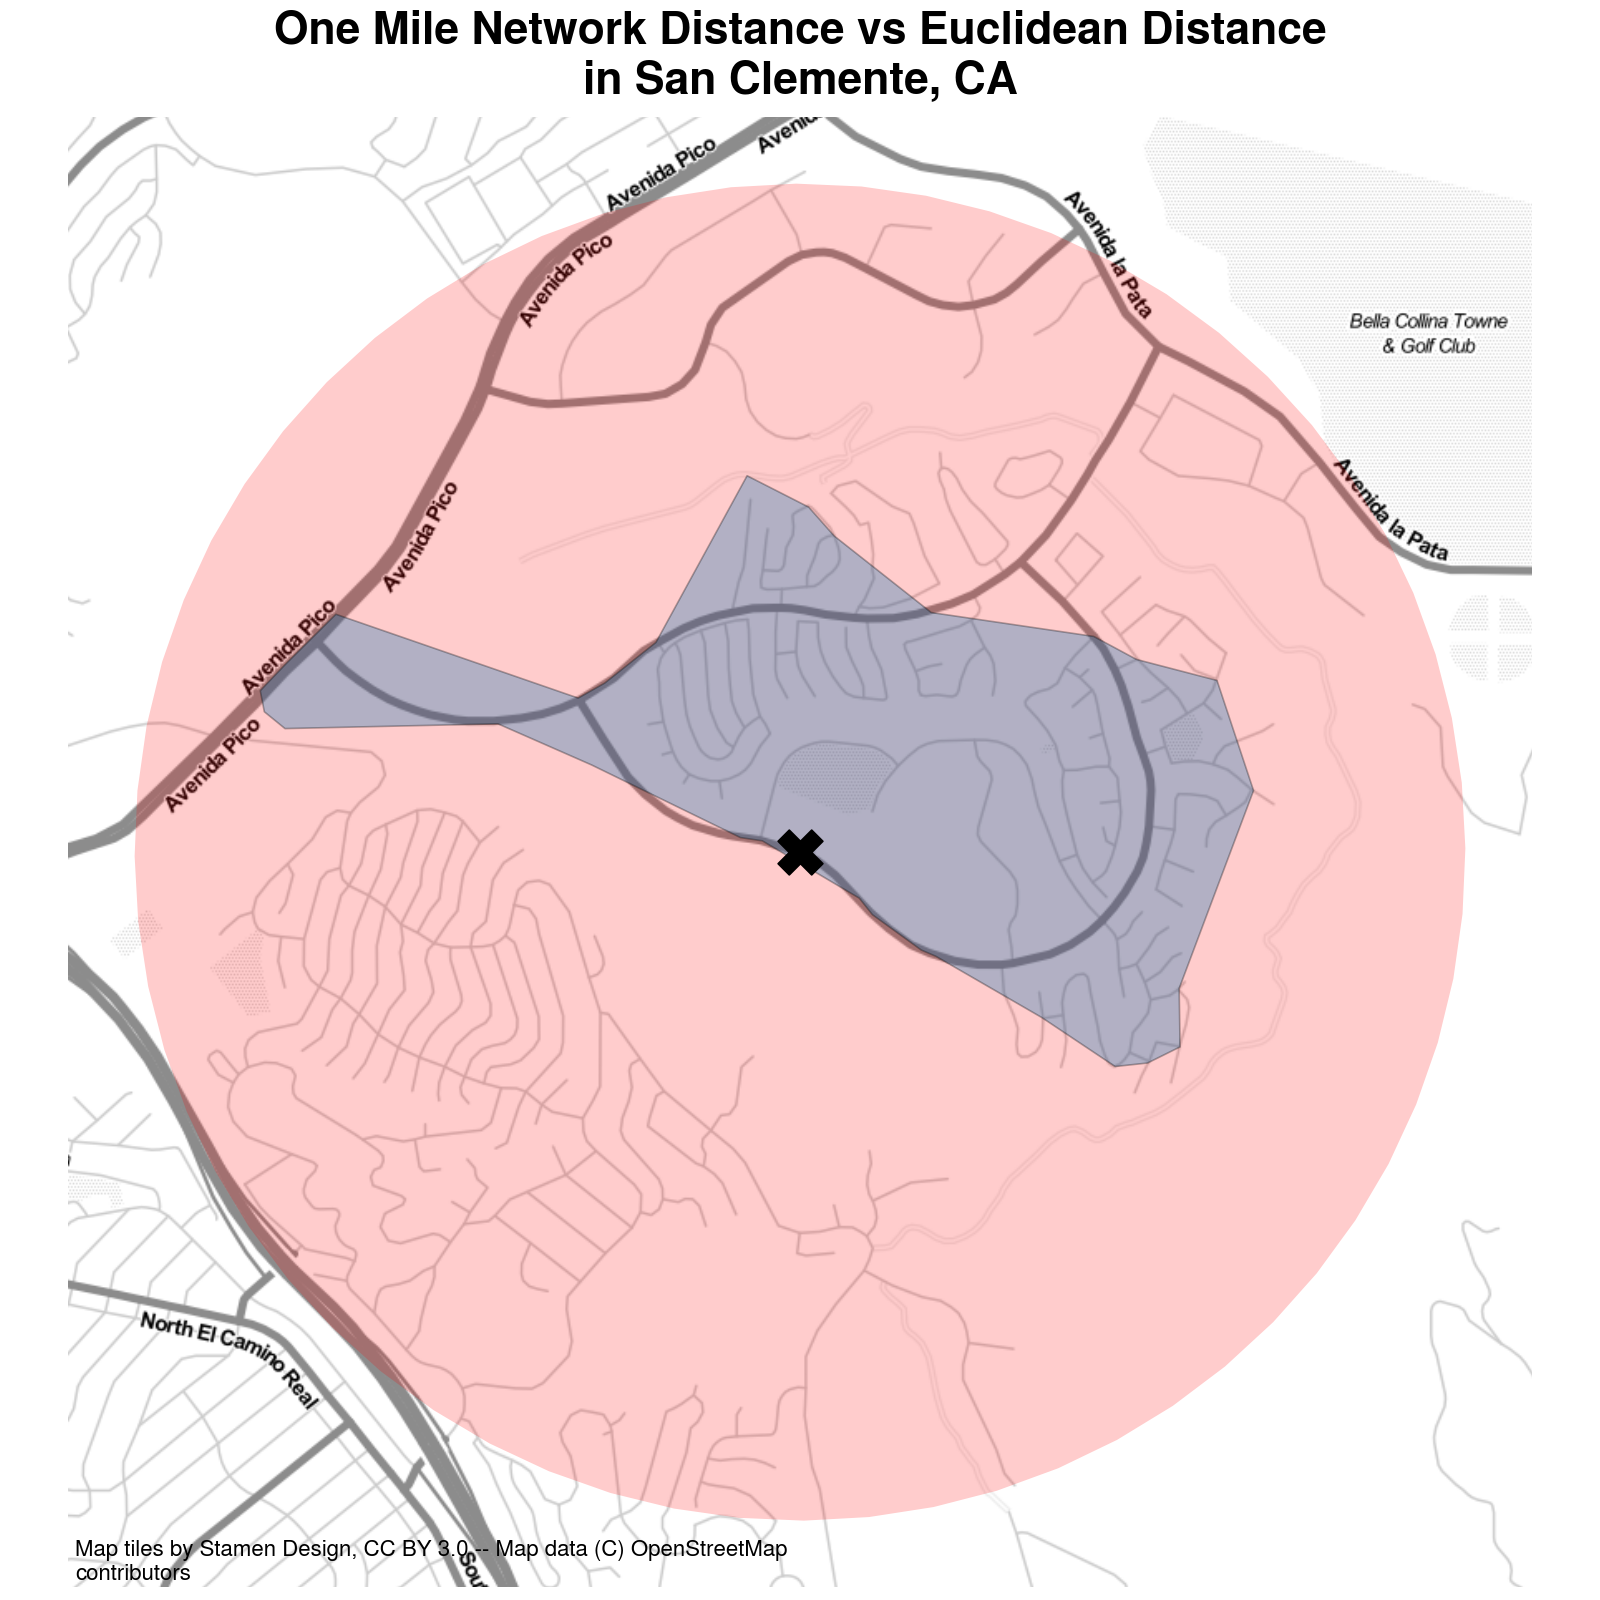
\includegraphics[width=0.49\textwidth,height=\textheight]{./figures/network_distance.png}\label{fig:distance_sd}}
\subfloat[Network Distance vs Euclidean
Distance]{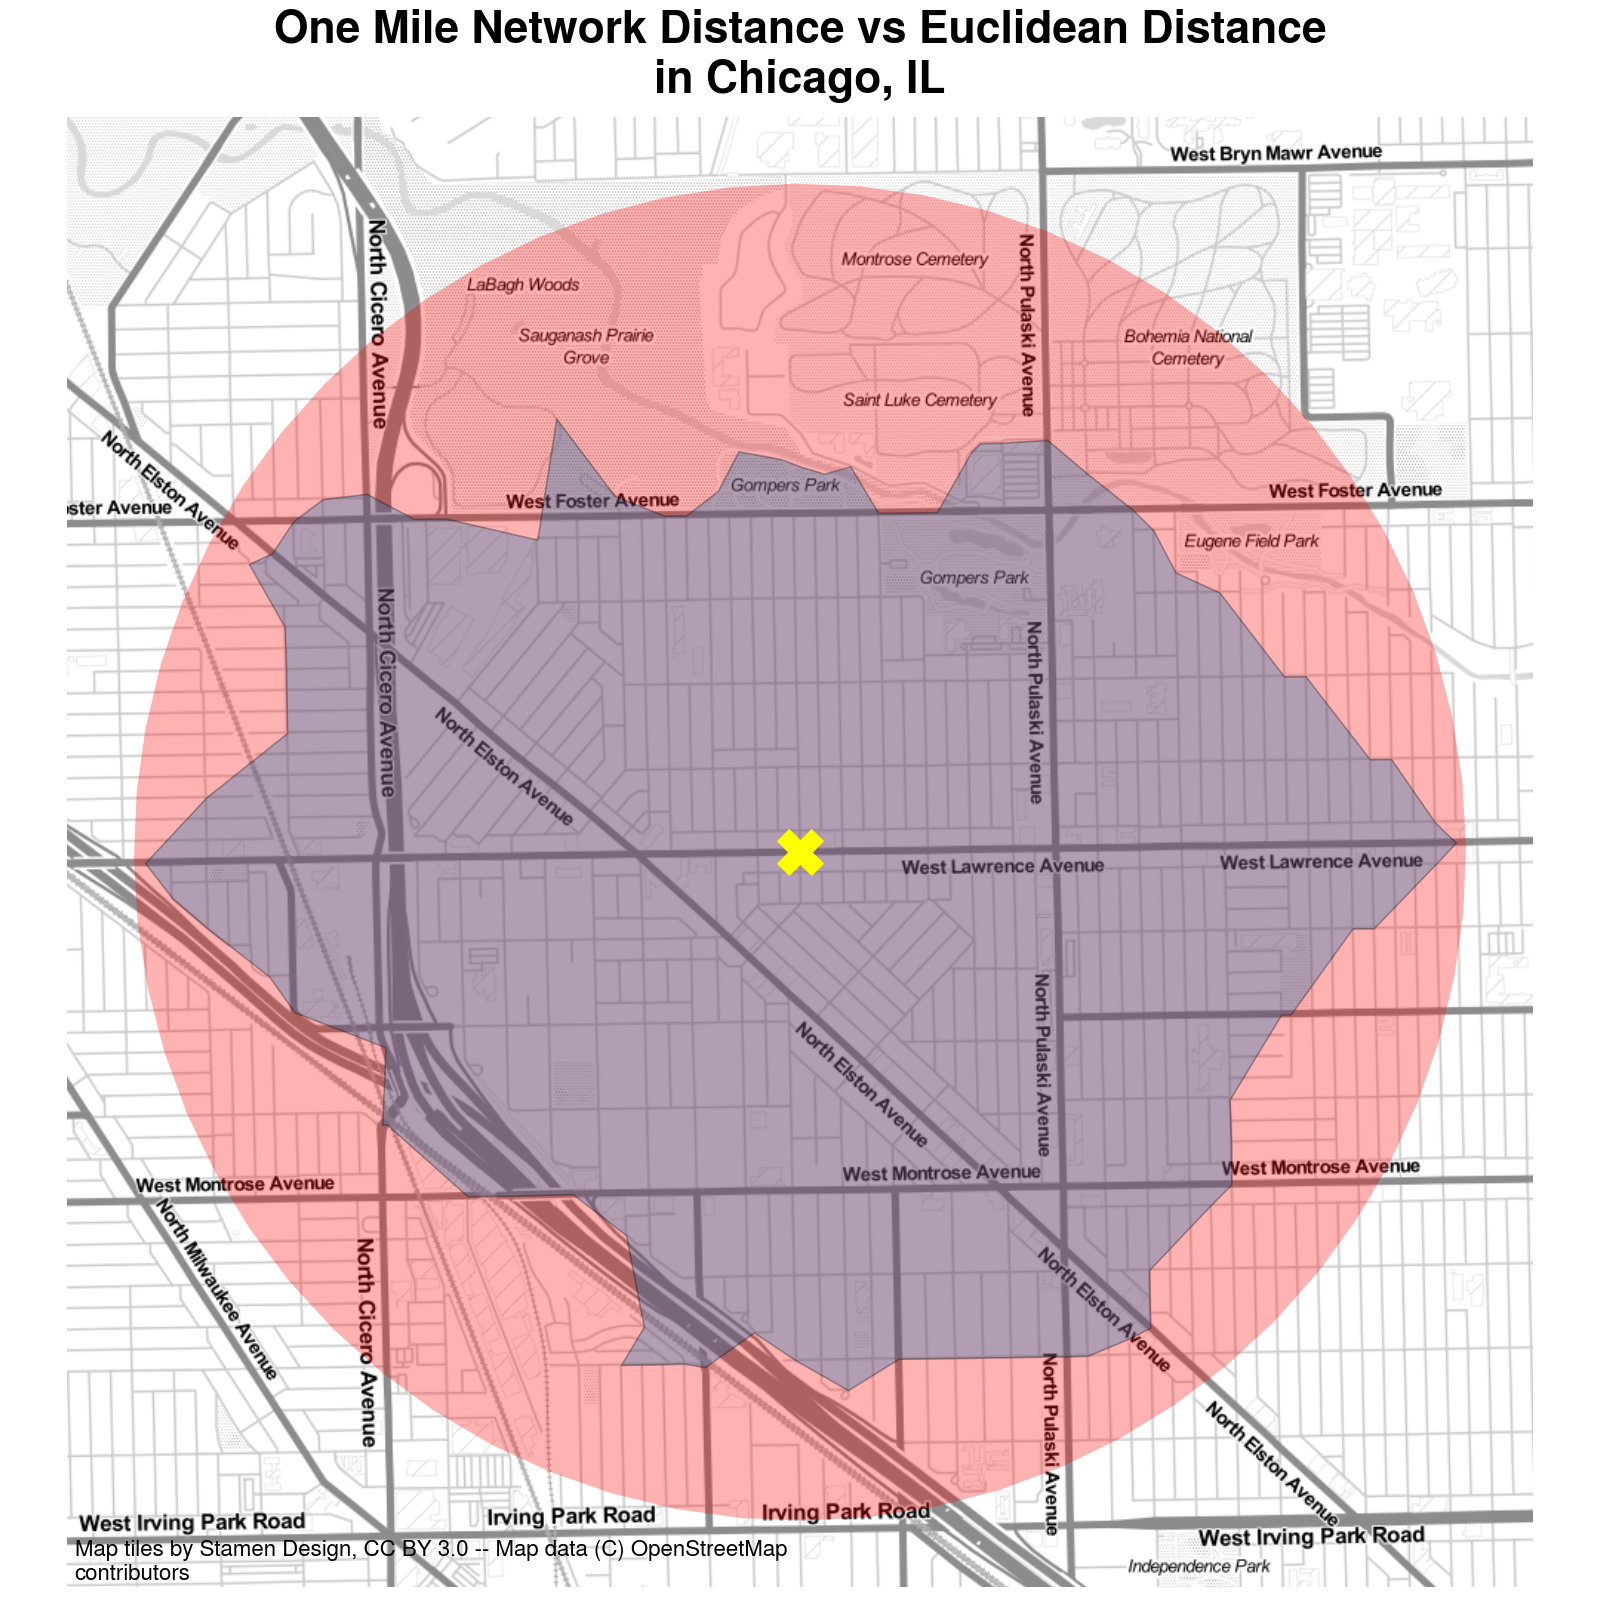
\includegraphics[width=0.49\textwidth,height=\textheight]{./figures/network_distance_chi.png}\label{fig:distance_chi}}

\caption[{Network Distance vs Euclidean Distance in Urban
Environments}]{Network Distance vs Euclidean Distance in Urban
Environments}

\label{fig:network_distance}

\end{pandoccrossrefsubfigures}

A depiction of the difference between network travel distance and ``as
the crow flies'' distance is shown in Figure~\ref{fig:network_distance}.
The figure shows an origin marked with an X in the center, and two
different polygons representing a one-mile travel distance using
different methods. The small polygon depicts the total extent accessible
from the origin point when traveling along the pedestrian network,
whereas the larger polygon depicts the 1-mile buffer representing
unconstrained travel. It is immediately apparent in the figure that
network-constrained travel covers a much smaller footprint than
euclidean distance in the depicted location. Furthermore, the pattern
appears to be influenced strongly by the street network and urban design
features that characterize the largely suburban region of the San Diego
metro area. Instead of a regular grid that facilitates travel in all
directions, the street network in Figure~\ref{fig:network_distance}
includes several insular patterns, cul-de-sacs, and 3-way intersections
that help channel traffic in certain directions rather than others.
Furthermore, the fact that some subdivisions have only a single entrance
makes clear how much further a person would need to travel to reach the
homes in certain regions (versus how much easier they appear to be
reached via the circular buffer).

Recent work by \citet{roberto2018SpatialProximity} shows the importance
of considering network distances when measuring segregation using both
simulated data and an empirical example in Pittsburgh, PA. That study
shows that segregation is consistently higher at all spatial scales when
the measure accounts for local network connectivity. As
\citet[p.~28]{roberto2018SpatialProximity} notes, ``even small positive
differences in the city-level results are meaningful and suggest that
physical barriers facilitate greater separation between ethnoracial
groups and higher levels of segregation.'' We agree with this assessment
and in what follows, we examine the magnitude of differences between
network and simple euclidean measures in detail for every metropolitan
region in the United States. Specifically, we expand upon prior work in
three different directions. First, we expand the geographic scope by
considering every metropolitan region in the United States, rather than
a case study of a single city. Second, we adopt a computational
inference framework that allows us to assess whether the observed
differences between the segregation measures are large enough that they
could not happen by chance. Finally, we explore the relationship between
differences in observed segregation and characteristics of the local
travel network.

\hypertarget{the-role-of-network-distance-in-segregation-measurement}{%
\section{The Role of Network Distance in Segregation
Measurement}\label{the-role-of-network-distance-in-segregation-measurement}}

We begin our analysis by computing two sets of segregation indices,
adopting the spatial information theory statistic \(\tilde{H}\) as our
measure of segregation. As \citet[p.~512]{reardon2008GeographicScale}
describe, ``the index \(\tilde{H}\) is a measure of how much less
diverse individuals' local environments are, on average, than is the
total population of region'', and reaches its maximum of 1 only when
``each individual's local environment is monoracial''. Here, our goal is
to test how sensitive the statistic is to different concepts of the
``local environment,'' with one concept adopting the simplified
assumption of euclidean-based distance measurements, and the other
requiring that distance be measured along a pedestrian transport
network.

\hypertarget{measuring-segregation-in-space}{%
\subsection{Measuring Segregation in
Space}\label{measuring-segregation-in-space}}

Following \citet{reardon2004MeasuresSpatial} we consider a spatial
region \(R\) populated by \(M\) racial groups indexed by \(m\), with
\(\tau\) and \(\pi\) as population density and proportion, respectively.
Here we diverge from the classical notation in the segregation
literature and instead adopt conventions more common in spatial
econometrics and geographic analysis. Doing so allows us to strengthen
the connection between similar concepts in different disciplines as well
as gain finer control over the definition of spatial relationships.
Since many spatial segregation measures are implemented in GIS and
spatial analysis software designed by geographers, clarifying this
connection can help ease interdisciplinary adoption and conversation
around spatial segregation measures.

Thus, we index locations within \(R\) as \(i\) and \(j\), and we
operationalize the concept of spatial relationships using a spatial
weights matrix \(W_{ij}\). By focusing on \(W_{ij}\), we are forced ``to
specify {[}our{]} underlying assumptions about socio-spatial
proximity'', following the call by
\citet[p.154]{reardon2004MeasuresSpatial} for analysis that ``compares
segregation levels based on different theoretical bases for defining
spatial proximity.'' Conceptually, the spatial weights matrix \(W_{ij}\)
is connectivity graph that defines the spatial relationship between
nodes \(i\) and \(j\), and the values \(w_{ij}\) encode the intensity of
the edge \(\bar{ij}\). Thus, the spatial weights matrix is a useful and
flexible representation of the local neighborhood environment because it
provides a generic data structure for encoding spatial relationships,
where any link function (\(\phi\), following the notation of
\citet{reardon2004MeasuresSpatial}) can be used to specify the proximity
between units. Formally,

\begin{equation}\protect\hypertarget{eq:weights}{}{
W_{ij} = \phi(D_{ij})
}\label{eq:weights}\end{equation}\\
Where \(\phi\) is a proximity weighting function and \(D\) is a matrix
containing pairwise distances for \(i\) and \(j\). Classically,
\(W_{ij}\) is typically created via binary connectivity between adjacent
units, but a wide variety of other continuous specifications are also
used in practice
\citep{getis2009SpatialWeights, rey2010PySALPython, halleckvega2015SLXMODEL},
such as the euclidean distance between observations, or various kernel
or distance-decay functions. Critically, the distance-weighting function
\(\phi\) is distinct from the concept of \emph{distance} (\(D\)),
itself, which could be measured in Euclidean/geodesic distance, minutes
of congested travel time, meters traveled along the sidewalk, or some
generalized measure of utility. Separating these two concepts allows us
to consider alternative distance metrics distinctly from alternative
decay functions. The local environment for a given feature \(y\) at
location \(i\) can then be measured by its \emph{spatial lag}, \(SL\),
defined as

\begin{equation}\protect\hypertarget{eq:lag}{}{
SL_i = \sum_j w_{ij} y_j
}\label{eq:lag}\end{equation}\\
In the spatial econometrics literature, it is common to exclude the
diagonal elements from \(W_{ij}\) to differentiate between focal effects
and spatial spillovers in regression models, but when the diagonal is
filled, then \(SL_i\) becomes a consummate measure of the local
environment at location \(i\).

To compute the spatial multigroup information theory index
\(\tilde{H}\), we first calculate local spatially-weighted population
proportions as

\begin{equation}\protect\hypertarget{eq:proportion}{}{
\tilde{\pi}_{im} = \frac{SL_{im}}{\sum^M_{m=1}{SL_{im}}}
}\label{eq:proportion}\end{equation}\\
The density at location \(i\) is

\begin{equation}\protect\hypertarget{eq:density}{}{
\tilde{\tau_i} = \frac{\sum^M_{m=1}{SL_{im}}}{\sum^M_{m=1}\sum^I_{i=1}{SL_{im}}}
}\label{eq:density}\end{equation}\\
The entropy of the local environment at each location \(\tilde{E}_i\) is

\begin{equation}\protect\hypertarget{eq:entropy}{}{
\tilde{E}_i = -\sum^M_{m=1}(\tilde{\pi}_{im})\log_M(\tilde{\pi}_{im})
}\label{eq:entropy}\end{equation}\\
where \(M\) indicates the number of groups in the population. Finally,

\begin{equation}\protect\hypertarget{eq:sit}{}{
\tilde{H} = 1-\frac{1}{TE} \sum^I \tilde{\tau_i}\tilde{E}_i
}\label{eq:sit}\end{equation}\\
where \(\tilde{H}\) is the spatial information theory index defined by
\citet{reardon2004MeasuresSpatial}. We perform all calculations using
the open-source Python package \texttt{segregation}
\citep{cortes2020OpensourceFramework}, distributed as part of the Python
Spatial Analysis Library (PySAL) \citep{rey2021PySALEcosystem}

\hypertarget{assessing-difference-between-distance-metrics}{%
\subsection{Assessing Difference Between Distance
Metrics}\label{assessing-difference-between-distance-metrics}}

To understand the implications of different parameterizations of space,
we use data blockgroup-level from the US Census American Community
Survey (ACS) 5-year sample (2013-2017) with four mutually-exclusive
racial groups (non-Hispanic white, non-Hispanic Black, Hispanic, and
Asian). Our sample contains data for 380 metropolitan Core Based
Statistical Areas (CBSAs) in the United States. Blockgroups are the
smallest geographic unit for which racial and ethnic data are available
in the ACS. To compute euclidean-based spatial segregation measures, our
distances are measured between blockgroup centroids; to compute
network-based spatial segregation measures, we first attach the
blockgroup centroids to the nearest intersection in the travel network,
then compute the shortest network-based path between each pair of
observations

Our data on street networks is collected from OpenStreetMap and the
shortest network path is computed using the Python package
\texttt{pandana} \citep{foti2012GeneralizedComputational}. To operate
efficiently on metropolitan-scale street networks, the pandana package
relies on a graph pre-processing technique known as contraction
hierarchies that simplifies the computation by removing inconsequential
nodes from consideration during the routing algorithm.

\hypertarget{constructing-comparable-indices}{%
\subsubsection{Constructing Comparable
Indices}\label{constructing-comparable-indices}}

In each metropolitan region, we proceed by creating two different
spatial weights matrices by varying the way distance is measured between
observations. In both matrices, the proximity-weighting function
\(\phi\) is a simple linear decay (triangular kernel) encoding a spatial
weight that decreases with distance up to a threshold of two kilometers,
outside of which observations no longer have an effect, (that is,
\(r=2000\)):

\begin{equation}\protect\hypertarget{eq:weighting_func}{}{
    \phi=
\begin{cases}
    1- \left( \frac{d_{ij}}{r} \right),& \text{if } d_{ij}\leq r \\ 
    0 & \text{otherwise}
\end{cases}
}\label{eq:weighting_func}\end{equation}\\

Between the two \(W\) matrices, however, we vary the input distance
matrix \(D\), between two concepts, euclidean distance and network
distance (where network distance is defined as the shortest path along
the pedestrian transportation network), \(W_{net}\), and \(W_{euc}\). In
both matrices the diagonal is set to one, indicating that there is no
spatial discount for the value located at observation \(i\). Using these
weights matrices \(W_{net}\) and \(W_{euc}\) to build local environments
for each metropolitan region in Equation~\ref{eq:weights} propagates the
two constructs through
Equations~\ref{eq:lag}, \ref{eq:proportion}, \ref{eq:density}, \ref{eq:entropy}, \ref{eq:sit},
yielding two segregation measures \(\tilde{H}_{net}\),
\(\tilde{H}_{euc}\) and, implicitly, a difference between the two,
\(\Delta_{\tilde{H}} = \tilde{H}_{net} - \tilde{H}_{euc}\). The relative
difference between segregation measures is the difference divided by the
euclidean measure
\(\Delta_{pct} = \frac{\Delta_{\tilde{H}}}{\tilde{H}_{euc}}\)

\hypertarget{inferential-framework}{%
\subsubsection{Inferential Framework}\label{inferential-framework}}

We assess the importance of considering network distance in segregation
measurement by adopting the inferential framework outlined in
\citet{rey2021ComparativeSpatial} and
\citet{cortes2020OpensourceFramework}. The approach leverages a
computational approach to statistical inference using random labelling
to compare the observed difference between the two segregation measures
(network versus euclidean) to a distribution of differences generated
from the same data. More specifically, the measures \(\tilde{H}_{net}\),
\(\tilde{H}_{euc}\) and \(\Delta_{\tilde{H}}\) are computed and recorded
for each metro region. As a result of this process, two ``spatialized''
versions of the metropolitan demographic composition are created, with
one dataset representing euclidean distances and the other representing
network-based distances.

We then create two synthetic datasets by pooling the input units from
both original datasets and reassigning them at random. For each
block-group, we randomly reassign the labels \((net,euc)\) to the
observed spatial lags from Equation~\ref{eq:lag}. Once all units have
been assigned to a group, the segregation measures are re-computed and
their difference taken. This process is repeated 10,000 iterations. By
comparing the observed difference between the two segregation measures
against a distribution of differences generated via synthetic datasets,
we can develop pseudo p-values based on a standard T-test. Our test in
this case measures the empirical likelihood of obtaining the observed
difference at random under the null hypothesis that the observed
difference is within the standard range of differences\footnote{Note
  this does not explicitly require the null \(\Delta_{\tilde{H}}=0\).
  Instead the ``null value'' is the mean of the simulated parameter
  distribution.}. The pseudo-\(p\) values represent probability of
obtaining results in which the simulated difference was greater than the
observed difference \(\Delta_{\tilde{H}}\).

\hypertarget{network-distance-is-an-important-consideration}{%
\subsection{Network Distance is an Important
Consideration}\label{network-distance-is-an-important-consideration}}

Although the correlation between planar and network based segregation
measures is \(\rho=0.987\), our results provide clear evidence that the
choice of appropriate distance metric plays an important role in the
computation of a spatial segregation index. In all but four cases, we
show that segregation is higher when measured according to network
distance than by pure euclidean distance\footnote{For each CBSA in our
  sample, our euclidean distances are based on UTM coordinate systems,
  with each region's data projected into its appropriate UTM zone.}
(none of the four cases are significant different from a random pooling
of the same data). Among the 380 CBAs in our dataset, 25.3\% have a
difference between euclidean and network-based segregation measures that
is signficant at the \(\alpha=0.05\) level, and 14.2\% of the CBSAs are
significant at the \(\alpha=0.01\) level. Descriptive statistics of the
differences between segregation measures in each metro are shown in
Table~\ref{tbl:diff_descriptives}, and a list of the 54 CBSAs
significant at the one percent level are listed in
Table~\ref{tbl:one_pct_diffs}. Among these 54 CBAS, eight metros are
located in California--twice the number of the next-most prevalent state
(Texas)

\begin{figure}
\hypertarget{fig:diff_hists}{%
\centering
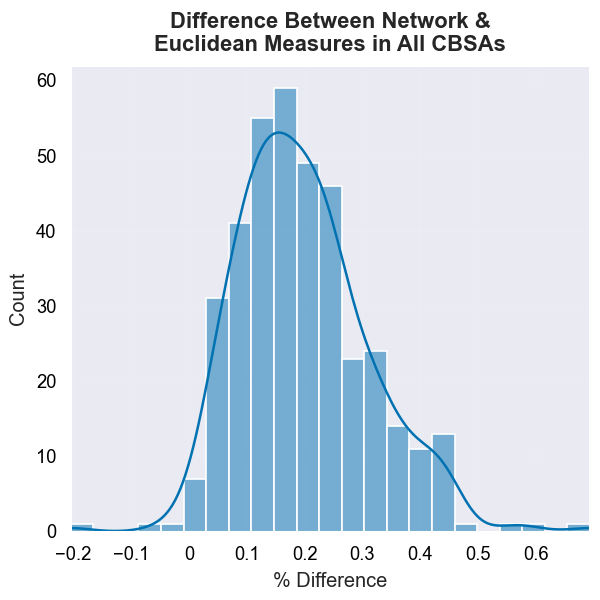
\includegraphics[width=0.4\textwidth,height=\textheight]{./figures/diff_hist.png}
\caption{Histogram of \% Differences in Segregation
Measures}\label{fig:diff_hists}
}
\end{figure}

\begin{table}[h]

\begin{center}
\begin{tabular}{lrrrr}
\hline
       &   planar\_measure &   network\_measure &   seg\_difference &   pct\_diff \\
\hline
 count &          380     &           380     &          380     &    380     \\
 mean  &            0.178 &             0.207 &            0.029 &      0.198 \\
 std   &            0.077 &             0.078 &            0.013 &      0.113 \\
 min   &            0.051 &             0.07  &           -0.053 &     -0.204 \\
 25\%   &            0.114 &             0.141 &            0.023 &      0.118 \\
 50\%   &            0.172 &             0.205 &            0.029 &      0.184 \\
 75\%   &            0.224 &             0.254 &            0.036 &      0.26  \\
 max   &            0.454 &             0.489 &            0.077 &      0.694 \\
\hline
\end{tabular}


\caption{Descriptive Statistics for Segregation Differences}
\label{tbl:diff_descriptives}
\end{center}
\end{table}

The shape of distribution of differences is approximately normal. While
the absolute difference between the two segregation measures in each
CBSA can appear small, the relative difference is often reasonably
large, with the network-based segregation measure approximately 20\%
higher than the euclidean-based measure on average. The largest relative
difference gets as high as 69\% (Carson City, NV).

\begin{table}
\centering
\caption{CBSAs with Highly Significant Differences in Segregation Measures}
\label{one_pct_diffs}
\begin{tabular}{lrrrrr}
\toprule
{} &  $\tilde{H}_{net}$ &  $\tilde{H}_{euc}$ &  $\Delta_{\tilde{H}}$ &  $\Delta_{pct}$ &  pseudo-$p$ \\
name                                         &                    &                    &                       &                 &             \\
\midrule
Anchorage, AK                                &              0.135 &              0.092 &                 0.043 &           0.470 &       0.002 \\
Atlanta-Sandy Springs-Alpharetta, GA         &              0.321 &              0.293 &                 0.028 &           0.095 &       0.001 \\
Austin-Round Rock-Georgetown, TX             &              0.174 &              0.152 &                 0.023 &           0.150 &       0.006 \\
Baltimore-Columbia-Towson, MD                &              0.331 &              0.284 &                 0.047 &           0.164 &       0.000 \\
Boston-Cambridge-Newton, MA-NH               &              0.254 &              0.228 &                 0.025 &           0.111 &       0.001 \\
Bridgeport-Stamford-Norwalk, CT              &              0.223 &              0.181 &                 0.042 &           0.235 &       0.001 \\
Charlotte-Concord-Gastonia, NC-SC            &              0.264 &              0.233 &                 0.032 &           0.136 &       0.000 \\
Chicago-Naperville-Elgin, IL-IN-WI           &              0.386 &              0.365 &                 0.021 &           0.057 &       0.000 \\
Cincinnati, OH-KY-IN                         &              0.315 &              0.262 &                 0.054 &           0.205 &       0.000 \\
Cleveland-Elyria, OH                         &              0.412 &              0.380 &                 0.033 &           0.086 &       0.004 \\
Columbus, OH                                 &              0.273 &              0.234 &                 0.039 &           0.168 &       0.001 \\
Dallas-Fort Worth-Arlington, TX              &              0.255 &              0.218 &                 0.037 &           0.171 &       0.000 \\
Denver-Aurora-Lakewood, CO                   &              0.197 &              0.176 &                 0.021 &           0.120 &       0.002 \\
Detroit-Warren-Dearborn, MI                  &              0.489 &              0.450 &                 0.038 &           0.085 &       0.000 \\
Hartford-East Hartford-Middletown, CT        &              0.313 &              0.264 &                 0.048 &           0.182 &       0.001 \\
Houston-The Woodlands-Sugar Land, TX         &              0.270 &              0.243 &                 0.028 &           0.114 &       0.000 \\
Indianapolis-Carmel-Anderson, IN             &              0.314 &              0.279 &                 0.034 &           0.123 &       0.008 \\
Kansas City, MO-KS                           &              0.294 &              0.266 &                 0.028 &           0.104 &       0.007 \\
Lansing-East Lansing, MI                     &              0.210 &              0.166 &                 0.044 &           0.268 &       0.003 \\
Las Vegas-Henderson-Paradise, NV             &              0.139 &              0.115 &                 0.023 &           0.202 &       0.000 \\
Los Angeles-Long Beach-Anaheim, CA           &              0.284 &              0.264 &                 0.019 &           0.072 &       0.000 \\
Louisville/Jefferson County, KY-IN           &              0.328 &              0.269 &                 0.060 &           0.222 &       0.000 \\
Miami-Fort Lauderdale-Pompano Beach, FL      &              0.354 &              0.323 &                 0.031 &           0.097 &       0.000 \\
Milwaukee-Waukesha, WI                       &              0.429 &              0.398 &                 0.031 &           0.079 &       0.008 \\
Minneapolis-St. Paul-Bloomington, MN-WI      &              0.209 &              0.177 &                 0.032 &           0.182 &       0.000 \\
New Haven-Milford, CT                        &              0.225 &              0.183 &                 0.042 &           0.230 &       0.001 \\
New Orleans-Metairie, LA                     &              0.260 &              0.227 &                 0.032 &           0.142 &       0.009 \\
New York-Newark-Jersey City, NY-NJ-PA        &              0.299 &              0.280 &                 0.019 &           0.067 &       0.000 \\
Oklahoma City, OK                            &              0.253 &              0.219 &                 0.034 &           0.155 &       0.006 \\
Olympia-Lacey-Tumwater, WA                   &              0.112 &              0.077 &                 0.035 &           0.456 &       0.004 \\
Peoria, IL                                   &              0.351 &              0.288 &                 0.063 &           0.218 &       0.004 \\
Philadelphia-Camden-Wilmington, PA-NJ-DE-MD  &              0.326 &              0.302 &                 0.024 &           0.080 &       0.000 \\
Phoenix-Mesa-Chandler, AZ                    &              0.209 &              0.182 &                 0.027 &           0.149 &       0.000 \\
Pittsburgh, PA                               &              0.280 &              0.225 &                 0.055 &           0.245 &       0.000 \\
Portland-Vancouver-Hillsboro, OR-WA          &              0.118 &              0.095 &                 0.024 &           0.249 &       0.001 \\
Redding, CA                                  &              0.120 &              0.084 &                 0.036 &           0.431 &       0.004 \\
Riverside-San Bernardino-Ontario, CA         &              0.169 &              0.144 &                 0.025 &           0.171 &       0.000 \\
Rochester, NY                                &              0.316 &              0.274 &                 0.042 &           0.152 &       0.003 \\
Sacramento-Roseville-Folsom, CA              &              0.152 &              0.129 &                 0.023 &           0.177 &       0.000 \\
Salt Lake City, UT                           &              0.146 &              0.121 &                 0.026 &           0.212 &       0.007 \\
San Antonio-New Braunfels, TX                &              0.231 &              0.200 &                 0.031 &           0.154 &       0.000 \\
San Diego-Chula Vista-Carlsbad, CA           &              0.204 &              0.184 &                 0.019 &           0.105 &       0.009 \\
San Francisco-Oakland-Berkeley, CA           &              0.167 &              0.154 &                 0.014 &           0.089 &       0.008 \\
Santa Rosa-Petaluma, CA                      &              0.118 &              0.088 &                 0.030 &           0.342 &       0.005 \\
Seattle-Tacoma-Bellevue, WA                  &              0.130 &              0.107 &                 0.023 &           0.217 &       0.000 \\
Springfield, MA                              &              0.312 &              0.256 &                 0.056 &           0.217 &       0.000 \\
St. Louis, MO-IL                             &              0.390 &              0.356 &                 0.034 &           0.095 &       0.005 \\
Stockton, CA                                 &              0.132 &              0.104 &                 0.027 &           0.262 &       0.009 \\
Tallahassee, FL                              &              0.196 &              0.146 &                 0.050 &           0.346 &       0.005 \\
Tampa-St. Petersburg-Clearwater, FL          &              0.239 &              0.213 &                 0.026 &           0.124 &       0.002 \\
Toledo, OH                                   &              0.268 &              0.218 &                 0.050 &           0.231 &       0.001 \\
Virginia Beach-Norfolk-Newport News, VA-NC   &              0.206 &              0.161 &                 0.045 &           0.277 &       0.000 \\
Washington-Arlington-Alexandria, DC-VA-MD-WV &              0.240 &              0.220 &                 0.020 &           0.092 &       0.001 \\
Worcester, MA-CT                             &              0.200 &              0.156 &                 0.044 &           0.281 &       0.001 \\
\bottomrule
\end{tabular}
\end{table}

\hypertarget{network-characteristics-and-segregation-differences}{%
\section{Network Characteristics and Segregation
Differences}\label{network-characteristics-and-segregation-differences}}

\hypertarget{metropolitan-travel-infrastructure-as-a-network-graph}{%
\subsection{Metropolitan Travel Infrastructure as a Network
Graph}\label{metropolitan-travel-infrastructure-as-a-network-graph}}

The travel infrastructure in a metropolitan region serves as its
skeleton for both urban development and social interactions. For
decades, scholars have worked to quantify the aspects of urban form that
help explain behaviors such as travel mode choice
\citep[\citet{ewing2010TravelBuilt}]{crane2000InfluenceUrban, clifton2008QuantitativeAnalysis, ewing2009MeasuringUnmeasurable}.
A recent evolution of this work is the conception of a travel network as
a formal graph structure
\citep{boeing2018PlanarityStreet, boeing2018MorphologyCircuity, fleischmann2021MethodologicalFoundation, fleischmann2018MeasuringUrban},
and a set of software tools that facilitate its analysis
\citep{boeing2016OSMnxNew, fleischmann2019MomepyUrban}.

\hypertarget{measuring-graph-structure}{%
\subsection{Measuring Graph Structure}\label{measuring-graph-structure}}

We use OSMNx and Momepy to create measures of the pedestrian travel
network collected from OpenStreetMap.

\hypertarget{graph-topology-and-segregation-differences}{%
\subsection{Graph Topology and Segregation
Differences}\label{graph-topology-and-segregation-differences}}

To understand how urban design decisions such as the topology of the
travel network may impact the ability for residents to interact (as
measured by the segregation index), we regress the difference in
measured segregation on measures of the network graph structure.

Our two-value test is doing a good job (i.e., it is picking up a
difference)

The ps\_inter is an interaction term between the planar\_measure and
whether the two-value test was significant. This tells us that the slope
is larger for those cities where the difference in the two-value test is
significant.

The pct difference generally declines with the overall level of
segregation and network size (as measured by street\_length) althoug the
latter association appears to be driven by the places with the
significant two-value tests

\hypertarget{discussion}{%
\section{Discussion}\label{discussion}}

There are two additional parameters worth exploring: the distance-decay
function \(\phi\), and the radius that defines the extent of the local
environment \(r\).

\hypertarget{conclusion}{%
\section{Conclusion}\label{conclusion}}

In the segregation literature, the importance of \emph{space} has long
been recognized, but a full grasp of its implications still eludes
researchers. In this paper, we show that when considering the role of
transportation infrastructure in segregation measurement, we obtain
substantially different results than classic spatial approaches that
adopt euclidean measurements.

In future work, this research could be extended in several directions

One promising direction is the consideration of alternative impedance
measures when calculating shortest-path distances along the travel
network. In the present study, we assume a constant rate of travel
consistent with the average walking pace, and that impedance is
reflected by graph distance alone. Alternative constructs could include
elevation along with distance to get a more complete measure of the
effort required to traverse by foot or bicycle. Similarly, the travel
network could also be extended to include public transportation or
(potentially congested) automobile travel. These considerations would
require extensive additional data, which may limit the capacity for
cross-sectional comparisons, but would also provide insight into
alternative concepts of space and distance.

Another important avenue for further work is the blending of multiple
graphs for a more complete understanding of multi-contextual
segregation. For example children who live in a given neighborhood are
simultaneously embedded in local neighborhood contexts, school catchment
boundaries, and other local institutions such as religious and community
organizations. Each of these contexts have partially-overlapping,
occasionally nested, and often imperfectly-defined geographic
boundaries, a full synthesis of which requires the development of new
methods that integrate across these contexts
\citep{galster2001NatureNeighbourhood, galster2019making}. As one
example, \citet{wolf2021SpatiallyEncouraged} provides a technique for
blending multiple graphs together, one spatial and one aspatial, and
similar methods could be possibly used to integrate multiple contexts.
Work along these lines would also help address the call by
\citet[p.~156]{reardon2004MeasuresSpatial} for metrics that help
understand bridges across social networks

\hypertarget{references}{%
\section{References}\label{references}}

\setstretch{1}

  \bibliography{paper-seg\_networks.bib}

\end{document}
